\documentclass{beamer}
\usepackage[utf8]{inputenc}
\usepackage[french]{babel}
\usepackage{hyperref}
\usepackage{fontawesome5}
\usepackage{caption}
\usepackage[absolute,overlay]{textpos}

\usepackage{tikz}
\usetikzlibrary{positioning}
\usepackage{siunitx}
\usepackage{xcolor}
\usepackage{lmodern}

\usetheme{metropolis}

% Couleurs noires partout
\definecolor{black}{RGB}{0,0,0}
\setbeamercolor{normal text}{fg=black,bg=white}
\setbeamercolor{frametitle}{fg=black,bg=white}
\setbeamercolor{title}{fg=black}
\setbeamercolor{subtitle}{fg=black}
\setbeamercolor{author}{fg=black}
\setbeamercolor{date}{fg=black}
\setbeamercolor{section title}{fg=black}
\setbeamercolor{item}{fg=black}
\setbeamercolor{enumerate item}{fg=black}
\setbeamercolor{itemize item}{fg=black}
\setbeamercolor{itemize subitem}{fg=black}
\setbeamercolor{structure}{fg=black}
\setbeamercolor{progress bar}{fg=darkgray,bg=gray!30}

\hypersetup{
    colorlinks=true,
    linkcolor=black,      % Liens internes (table des matières par ex.)
    urlcolor=blue,        % Couleur des \href
    pdfborder={0 0 1}     % Bordure (0 0 1) = souligné, pas de cadre
}

% Macros
\newcommand{\NomPrenom}{Kervadec Mattéo}
\newcommand{\DateSoutenance}{18/06/2025}
% Définition d'une macrode bulle
\newcommand{\kpiBox}[3]{
  \begin{tikzpicture}[baseline]
    \node[draw=#3!80!black, fill=#3!10, rounded corners=5pt,
          minimum width=2.5cm, minimum height=1.5cm,
          text centered, line width=0.5pt, inner sep=6pt] (box) {
      \begin{tabular}{c}
        \large #2 \\
		\small #1
      \end{tabular}
    };
  \end{tikzpicture}
}

\newcommand{\logoEdeclic}{
	\begin{textblock*}{2cm}(9.5cm,0.5cm)
  		
\includegraphics[height=1cm]{../img/logo_e-declic.png}
	\end{textblock*}
}

% Macros Sommaire
\newcommand{\planLine}[4]{
  \ifnum#1=#2
    \item \hyperlink{#3}{\textbf{\large #4}}
  \else
    \item \hyperlink{#3}{#4}
  \fi
}
\newcommand{\planSlide}[1]{
  	\begin{frame}{Plan de la présentation}
  		\begin{center}
  			\begin{minipage}{1\textwidth}
				\begin{itemize}
      			\planLine{#1}{1}{organisation}{Qui est E-declic ?}
      			\planLine{#1}{2}{sujet}{Les missions et objectifs du stage}
      			\planLine{#1}{3}{environnement}{Environnement de travail}
      			\planLine{#1}{4}{realisation}{Solutions apportées aux projets}
      			\planLine{#1}{5}{conclusion}{Conclusion}
	    		\end{itemize}
  		\end{minipage}
	\end{center}
	\vfill
	\end{frame}
}



% Compteur de page
\newcounter{currentframenumber}
\newcounter{totalframenumber}

% Pied de page
\setbeamertemplate{footline}{
  	\setcounter{currentframenumber}{\insertframenumber}
	\addtocounter{currentframenumber}{-1}
	\setcounter{totalframenumber}{\inserttotalframenumber}
  	\addtocounter{totalframenumber}{-1}

  	% Progress bar
  	\leavevmode%
  	\hbox{%
    		\begin{beamercolorbox}[wd=\paperwidth,ht=0.8ex,dp=0ex,left]{progress bar}
      		\rule{\dimexpr\paperwidth * \thecurrentframenumber{} / \thetotalframenumber}{0.8ex}
    		\end{beamercolorbox}%
  	}

	% Footer (infos + pagination)
  	\hbox{%
    		\begin{beamercolorbox}[wd=0.85\paperwidth,ht=3.5ex,dp=1ex,left]{author in head/foot}
		 	\hspace{1em}\footnotesize \NomPrenom \hspace{1em} | \hspace{1em} \DateSoutenance
	    \end{beamercolorbox}%
    		\begin{beamercolorbox}[wd=0.15\paperwidth,ht=3.5ex,dp=1ex,right]{author in head/foot}
			\footnotesize \thecurrentframenumber{} / \thetotalframenumber\hspace{1em}
    		\end{beamercolorbox}%
  	}

  	% Petit ajustement en bas
  	\vskip0pt%
}

% Information meta
\title[IUT Lannion -- Soutenance Stage]{E-declic - Soutenance de stage \\ \normalsize du 07/04/2025 au 01/06/2025 (8 semaines)}
\author{\NomPrenom}
\institute{IUT de Lannion -- Département Informatique}
\date{\DateSoutenance}

\begin{document}

% Page de garde
\begin{frame}[plain]
	\begin{minipage}[t]{0.75\textwidth}
    		\titlepage
  	\end{minipage}
	\begin{textblock*}{2cm}(11cm,0.5cm)
    		
\includegraphics[height=1.5cm]{../img/logo_iut.png}
	\end{textblock*}
\end{frame}

\planSlide{1}

% === ORGANISATION ===
\begin{frame}[label=organisation]{Qui est E-declic ?}
	\logoEdeclic

	\begin{beamercolorbox}[wd=\paperwidth,ht=1.5em,dp=0.5em,leftskip=0.5cm]{section in head/foot}
  		\large \textbf{Informations générales}
	\end{beamercolorbox}
	\vspace{0.5em}
	\begin{center}
  		\begin{minipage}{0.9\textwidth}
    			\begin{itemize}
      			\item Dénomination sociale : E-declic
				\item Nationalité : Française
      			\item Forme juridique : SARL
      			\item Secteur d'activité : Technologies de l'Information et de la Communication (TIC)
      			\item Taille : Petite moyenne entreprise (6 à 9 salariés)
    			\end{itemize}
  		\end{minipage}
	\end{center}
	\vfill
\end{frame}

\begin{frame}{Qui est E-declic ?}
	\logoEdeclic

	\begin{beamercolorbox}[wd=\paperwidth,ht=1.5em,dp=0.5em,leftskip=0.5cm]{section in head/foot}
  		\large \textbf{Localisation}
	\end{beamercolorbox}
	\vspace{0.5em}
	\begin{center}
  		\begin{minipage}{0.9\textwidth}
			\begin{figure}[t]
  				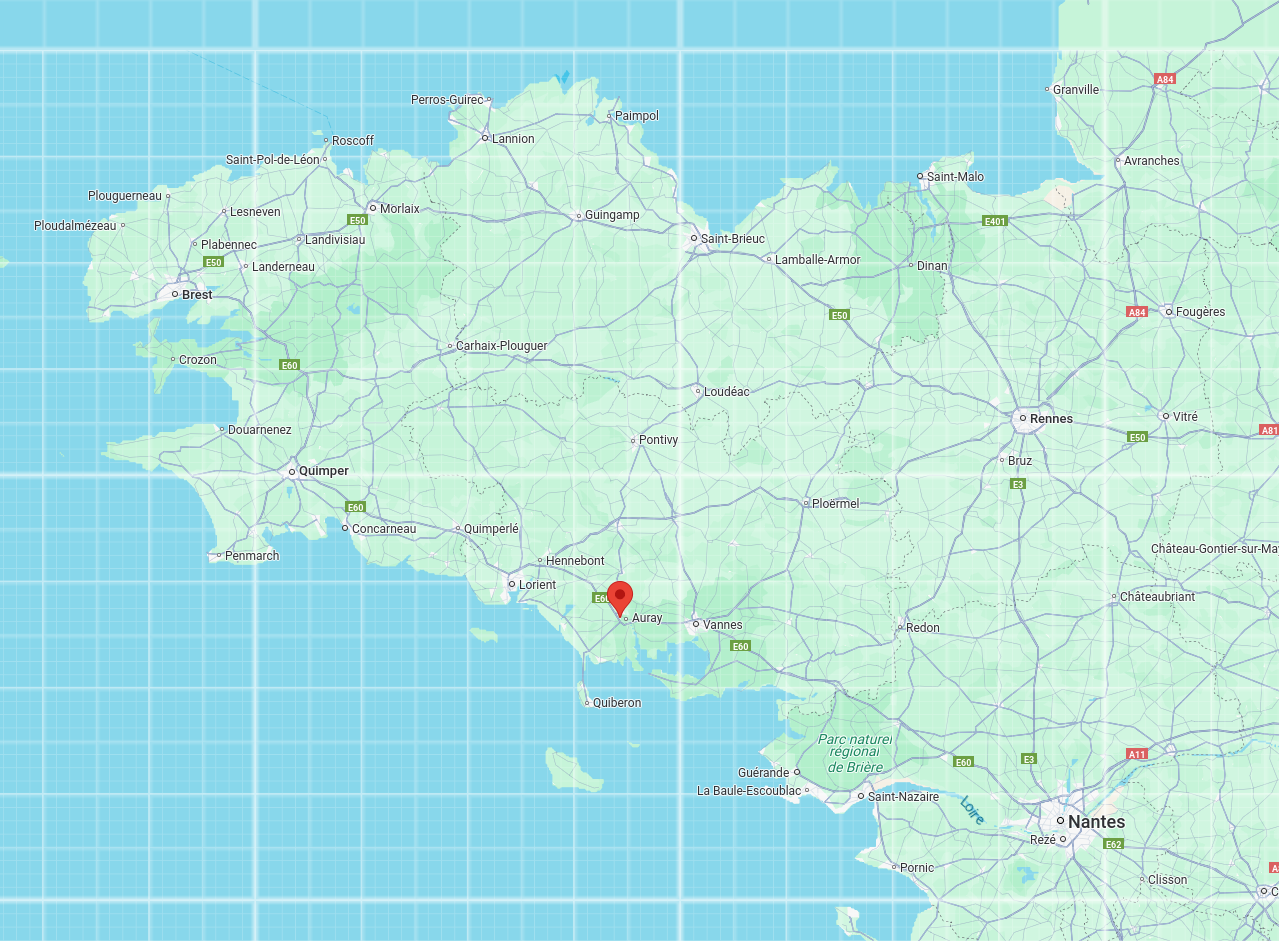
\includegraphics[height=5.5cm]{../img/localisation.png}
				\caption{				
  					\href{https://maps.app.goo.gl/11j9ZHKrL6TVrdYB6}{\underline{32 rue du Danemark}}.\\
  					\textit{Source : Google Maps.}
				}
  				\label{fig:localisation}
  			\end{figure}
  		\end{minipage}
	\end{center}
	\vfill
\end{frame}

\begin{frame}{Qui est E-declic ?}
	\logoEdeclic

	\begin{beamercolorbox}[wd=\paperwidth,ht=1.5em,dp=0.5em,leftskip=0.5cm]{section in head/foot}
  		\large \textbf{Activités et finalité}
	\end{beamercolorbox}
	\vspace{0.5em}
	\begin{center}
  		\begin{minipage}{0.9\textwidth}
			\begin{itemize}
  				\item Activité principale : Programmation informatique (NAF : 6201Z)
  				\item Services proposés :
  				\begin{itemize}
  					\item Développement de site web
  					\item Maintenance informatique
  					\item Communication graphique
  					\item Organisation d'évènements
  				\end{itemize}
  				\item Finalités : Apporter des solutions numériques et évènementielles sur mesure aux entreprises
  			\end{itemize}
  		\end{minipage}
	\end{center}
	\vfill
\end{frame}

\begin{frame}{Qui est E-declic ?}
	\logoEdeclic

	\begin{beamercolorbox}[wd=\paperwidth,ht=1.5em,dp=0.5em,leftskip=0.5cm]{section in head/foot}
  		\large \textbf{Chiffres clés}
	\end{beamercolorbox}
	\vspace{0.5em}
	\begin{center}
  		\begin{minipage}{0.9\textwidth}
			\kpiBox{Chiffre d'Affaires}{\num{1250000}~€}{blue}
			\kpiBox{Projets réalisés}{$+ 500$}{red}
			%\kpiBox{Rentabilité}{\num{5.49}~\%}{orange}
			%\kpiBox{Financière}{\num{21.68}~\%}{teal}
			\kpiBox{Salariés}{6 à 9}{green}
  		\end{minipage}
	\end{center}
	\vfill
\end{frame}

\begin{frame}{Qui est E-declic ?}
	\logoEdeclic
	
	\begin{beamercolorbox}[wd=\paperwidth,ht=1.5em,dp=0.5em,leftskip=0.5cm]{section in head/foot}
  		\large \textbf{Besions et objectifs}
	\end{beamercolorbox}
	\vspace{0.5em}
	\begin{center}
  		\begin{minipage}{0.9\textwidth}
			\textbf{Besoins}
			\begin{itemize}
				\item Répondre aux demandes en développement web
				\item Créer des outils numériques sur mesure
			\end{itemize}
	
			\textbf{Objectifs}
			\begin{itemize}
				\item Assurer la qualité et la fiabilité des services
				\item Maintenir une rentabilité positive
				\item Fidéliser la clientèle locale et régionale
			\end{itemize}
  		\end{minipage}
	\end{center}
	\vfill
\end{frame}

\begin{frame}{Qui est E-declic ?}
	\logoEdeclic
	
	\begin{beamercolorbox}[wd=\paperwidth,ht=1.5em,dp=0.5em,leftskip=0.5cm]{section in head/foot}
  		\large \textbf{Moyen de coordination et de direction}
	\end{beamercolorbox}
	\vspace{0.5em}
	\begin{center}
  		\begin{minipage}{0.9\textwidth}
			\begin{figure}[t]
  				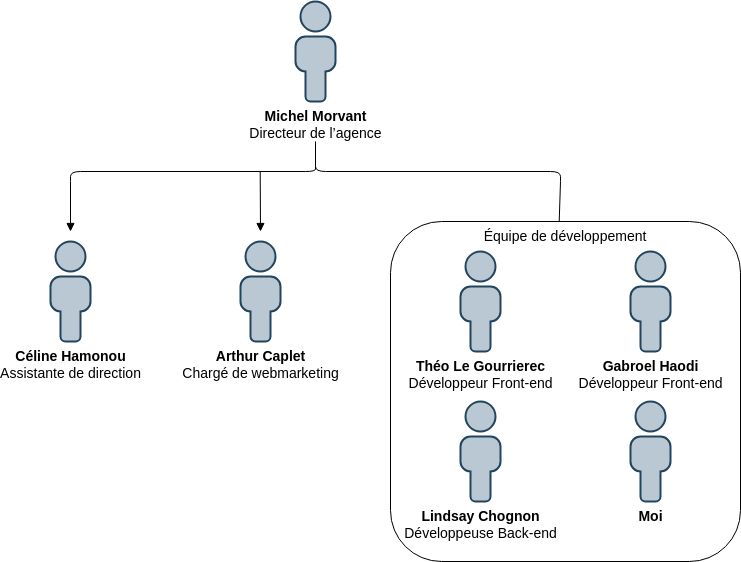
\includegraphics[height=5.5cm]{../img/coordination.png}
  				\caption{
    					\href{https://www.e-declic.com/agence-web/equipe/}{\underline{Moyen de coordination}}.\\
    					\textit{Source : Mattéo Kervadec}
  				}
  				\label{fig:coordination}
  			\end{figure}
  		\end{minipage}
	\end{center}
	\vfill
\end{frame}

\planSlide{2}

% === SUJET DE STAGE ===
\begin{frame}[label=sujet]{Les missions et objectifs du stage}

	\begin{beamercolorbox}[wd=\paperwidth,ht=1.5em,dp=0.5em,leftskip=0.5cm]{section in head/foot}
  		\large \textbf{Sujet de stage}
	\end{beamercolorbox}
	\vspace{0.2em}
	
	\begin{center}
  		\begin{minipage}{0.9\textwidth}				

    		\hspace{0.5cm} \small Le stage de \textbf{développement d'applications web} se concentrera sur la création, l'amélioration, et la maintenance d'applications web \textbf{interactives}, \textbf{responsive}, et \textbf{sécurisées}. Le stagiaire participera activement au développement de fonctionnalités côté client (\textbf{frontend}) et côté serveur (\textbf{backend}), selon les besoins du projet, tout en \textbf{respectant les bonnes pratiques} en matière de \textbf{code}, de \textbf{performance} et de \textbf{sécurité}. Le stagiaire \textbf{sera impliqué} dans plusieurs étapes du cycle de \textbf{développement} d'une application web, de la \textbf{planification} et \textbf{conception} à l'implémentation et aux \textbf{tests}. Le projet pourra inclure la \textbf{création de nouvelles applications}, l'\textbf{ajout de fonctionnalités} à des systèmes existants, ou encore la \textbf{refonte d'applications} pour améliorer leur performance et leur expérience utilisateur.
				
  		\end{minipage}
	\end{center}
	\vfill
\end{frame}

\begin{frame}{Les missions et objectifs du stage}

	\begin{beamercolorbox}[wd=\paperwidth,ht=1.5em,dp=0.5em,leftskip=0.5cm]{section in head/foot}
  		\large \textbf{Sujet de stage}
	\end{beamercolorbox}
	\vspace{0.2em}
	
	\begin{center}
  		\begin{minipage}{1\textwidth}				

    			\faLaptopCode\ \textbf{Développement web full-stack :}
      		\begin{itemize}
        			\item Frontend \& Backend
        			\item Interactives \& Responsives
      		\end{itemize}

    			\vspace{0.5em}
    			\faCheckCircle\ \textbf{Bonnes pratiques :}
      		\begin{itemize}
        			\item Programmation, performance et sécurité
      		\end{itemize}

    			\vspace{0.5em}
    			\faProjectDiagram\ \textbf{Cycle de développement :}
      		\begin{itemize}
        			\item Planification → Conception → Implémentation → Tests
      		\end{itemize}

    			\vspace{0.5em}
    			\faTasks\ \textbf{Missions possibles :}
      		\begin{itemize}
        			\item Nouvelles apps, fonctionnalités, refonte
      		\end{itemize}
  		\end{minipage}
	\end{center}
	\vfill
\end{frame}

\begin{frame}{Les missions et objectifs du stage}

	Comment répondre aux besoins spécifiques de réservation en ligne pour des hébergements touristiques via une application web, et permettre à l’agence E-declic d’élargir son offre de services ?
			
	\begin{center}
  		\begin{minipage}{0.9\textwidth}
  			\vspace{10cm}
  		\end{minipage}
	\end{center}
	\vfill
\end{frame}

\begin{frame}{Les missions et objectifs du stage}

	Comment répondre aux besoins spécifiques de réservation en ligne pour des hébergements touristiques via une application web, et permettre à l’agence E-declic d’élargir son offre de services ?
			
	\begin{center}
  		\begin{minipage}{0.9\textwidth}
			\begin{beamercolorbox}[wd=\paperwidth,ht=1.5em,dp=0.5em,leftskip=0.5cm]{section in head/foot}
  				\large \textbf{Missions confiées} - \href{https://github.com/Matteo-K/Soutenance_E-delic/blob/main/pdf/cc-painspizzas-camping.pdf}{\underline{(Lien du pdf sur github)}}
			\end{beamercolorbox}
			\begin{itemize}
				\item Gestion d'hébergements
				\item Gestion d'utilisateur
				\item Gestion du E-commerce
				\begin{itemize}
					\item Gestion de produit
					\item Gestion du panier
					\item Gestion du paiement
					\item \textbf{Gestion de la disponibilité des produits}
				\end{itemize}
				\item Gestion de l'administration
			\end{itemize}
  		\end{minipage}
  		\vspace{1cm}
	\end{center}
	\vfill
\end{frame}

\begin{frame}{Les missions et objectifs du stage}

	Comment répondre aux besoins spécifiques de réservation en ligne pour des hébergements touristiques via une application web, et permettre à l’agence E-declic d’élargir son offre de services ?
			
	\begin{center}
  		\begin{minipage}{0.9\textwidth}
			\begin{beamercolorbox}[wd=\paperwidth,ht=1.5em,dp=0.5em,leftskip=0.5cm]{section in head/foot}
  				\large \textbf{Principales difficultés attendues}
			\end{beamercolorbox}
			
			\begin{itemize}
				\item Gestion multi-utilisateur → multi-rôles
				\item Gestion de la disponibilité des produits
				\begin{itemize}
					\item Gestion du produit
					\item Gestoin du panier
					\item Gestion des commandes
					\item Gestion de l'historique
				\end{itemize}
				\item Intégration du paiement via stripe
			\end{itemize}
  			\vspace{1cm}
  		\end{minipage}
	\end{center}
	\vfill
\end{frame}

\planSlide{3}

% === ENVIRONNEMENT ===
\begin{frame}[label=environnement]{Environnement de travail}
	\begin{beamercolorbox}[wd=\paperwidth,ht=1.5em,dp=0.5em,leftskip=0.5cm]{section in head/foot}
  		\large \textbf{Outils utilisés}
	\end{beamercolorbox}
	\vspace{0.5em}
	\begin{center}
  		\begin{minipage}{0.9\textwidth}
  			\begin{columns}[T, onlytextwidth]
        			\column{0.48\textwidth}
        				
        				% Looping
        				\begin{minipage}[t][2cm][t]{\linewidth}
        					\raggedright
         				
\includegraphics[width=1.35cm, height=0.75cm, keepaspectratio]{../img/logo_looping.png} 
         				\hspace{0.1cm} \textbf{Looping} \\ 
         				Gestionnaire de MCD et modélisation
          		  	\end{minipage}
          			\vspace{0.7em}
          			\pause
          			
          			% Figma
        				\begin{minipage}[t][2cm][t]{\linewidth}
        					\raggedright
          				
\includegraphics[height=0.75cm]{../img/logo_figma.png}
          				\hspace{0.95cm} \textbf{Figma} \\
          				Conception des maquettes UI/UX
          			\end{minipage}
          			\vspace{0.7em}
          			\pause
          		
          			% Windsurf	
          			\begin{minipage}[t][2cm][t]{\linewidth}
          				\raggedright
          				
\includegraphics[width=0.75cm, height=0.75cm]{../img/logo_windsurf.png}
          				\hspace{0.6cm} \textbf{Windsurf} \\ 
          				Monitoring des performances
          			\end{minipage}
          			\pause
          			
        			\column{0.48\textwidth}
        			
        				% Postman
        				\begin{minipage}[t][2cm][t]{\linewidth}
        					\raggedright
          				
\includegraphics[width=0.75cm, height=0.75cm]{../img/logo_postman.png}
          				\hspace{0.6cm} \textbf{Postman} \\
          				Tests des API
          			\end{minipage}
          			\vspace{0.7em}
          			\pause
          			
          			% Github
          			\begin{minipage}[t][2cm][t]{\linewidth}
          				\raggedright
          				
\includegraphics[width=0.75cm, height=0.75cm]{../img/logo_github.png}
          				\hspace{0.6cm} \textbf{Github} \\
          				Gestion du versioning et partage de fichiers
          			\end{minipage}
          			\vspace{0.7em}
          			\pause
          			
          			% Slack
          			\begin{minipage}[t][2cm][t]{\linewidth}
          				\raggedright
          				
\includegraphics[width=0.75cm, height=0.75cm]{../img/logo_slack.png}
          				\hspace{0.6cm} \textbf{Slack} \\
          				Messagerie instantanée
          			\end{minipage}

      		\end{columns}
  		\end{minipage}
	\end{center}
	\vfill
\end{frame}

\begin{frame}{Environnement de travail}
	\begin{beamercolorbox}[wd=\paperwidth,ht=1.5em,dp=0.5em,leftskip=0.5cm]{section in head/foot}
  		\large \textbf{Langages utilisés}
	\end{beamercolorbox}
	\vspace{0.5em}
	\begin{center}
		\begin{minipage}{0.9\textwidth}
  			\begin{columns}[T, onlytextwidth]
    				\column{0.48\textwidth}
    
    					\vspace{2.5em}
      				% Symfony
      				\begin{minipage}[t][2cm][t]{\linewidth}
        					\raggedright
        					
\includegraphics[height=0.75cm]{../img/logo_symfony.png}
        					\hspace{0.6cm} \textbf{Symfony} \\
        					Framework PHP MVC pour l'architecture backend
      				\end{minipage}
      				\vspace{0.7em}
          			\pause
      
      				% Twig
      				\begin{minipage}[t][2cm][t]{\linewidth}
        					\raggedright
        					
\includegraphics[height=0.75cm]{../img/logo_twig.png}
        					\hspace{0.6cm} \textbf{Twig} \\
        					Moteur de templates pour Symfony
      				\end{minipage}
          			\pause

    				\column{0.48\textwidth}
    
      				% Turbo / Stimulus
      				\begin{minipage}[t][2cm][t]{\linewidth}
        					\raggedright
        					\textbf{Turbo/Stimulus} \\
        					Interaction frontend et mises à jour dynamiques
      				\end{minipage}
      				\vspace{0.7em}
          			\pause
      
      				% Twig Components
      				\begin{minipage}[t][2cm][t]{\linewidth}
        					\raggedright
        					\textbf{Twig Components} \\
        					Représentation réutilisable des éléments d'interface
      				\end{minipage}
      				\vspace{0.7em}
          			\pause
      
      				% Autocomplete
      				\begin{minipage}[t][2cm][t]{\linewidth}
        					\raggedright
        					\textbf{Autocomplete} \\
        					Champ de saisie avec suggestions dynamiques
      				\end{minipage}
      
  			\end{columns}
		\end{minipage}
	\end{center}
	\vfill
\end{frame}

\begin{frame}[label=env]{Environnement de travail}
    \begin{beamercolorbox}[wd=\paperwidth,ht=1.5em,dp=0.5em,leftskip=0.5cm]{section in head/foot}
        \large \textbf{Moyens d'organisation du projet}
    \end{beamercolorbox}
    \vspace{0.5em}
    \begin{center}
\begin{minipage}{0.9\textwidth}
    \begin{itemize}
        \item \textbf{Méthode de travail :} gestion souple, sans cadre agile
        \item \textbf{Réunions :} point hebdomadaire (lundi 10h)
        \item \textbf{Suivi des tâches :} carnet de fonctionnalités
        \item \textbf{Gestion des incidents :} journal des problèmes et solutions
        \item \textbf{Communication :} échanges quotidiens et à distance via Slack
    \end{itemize}
\end{minipage}

    \end{center}
    \vfill
\end{frame}

\begin{frame}[label=env]{Environnement de travail}  
	\begin{beamercolorbox}[wd=\paperwidth,ht=1.5em,dp=0.5em,leftskip=0.5cm]{section in head/foot}
  		\large \textbf{Planning Gantt et organisation personnelle}
	\end{beamercolorbox}
	\vspace{0.5em}
	\begin{center}
		\begin{minipage}{0.9\textwidth}
			\begin{figure}[t]
  				\centering
  				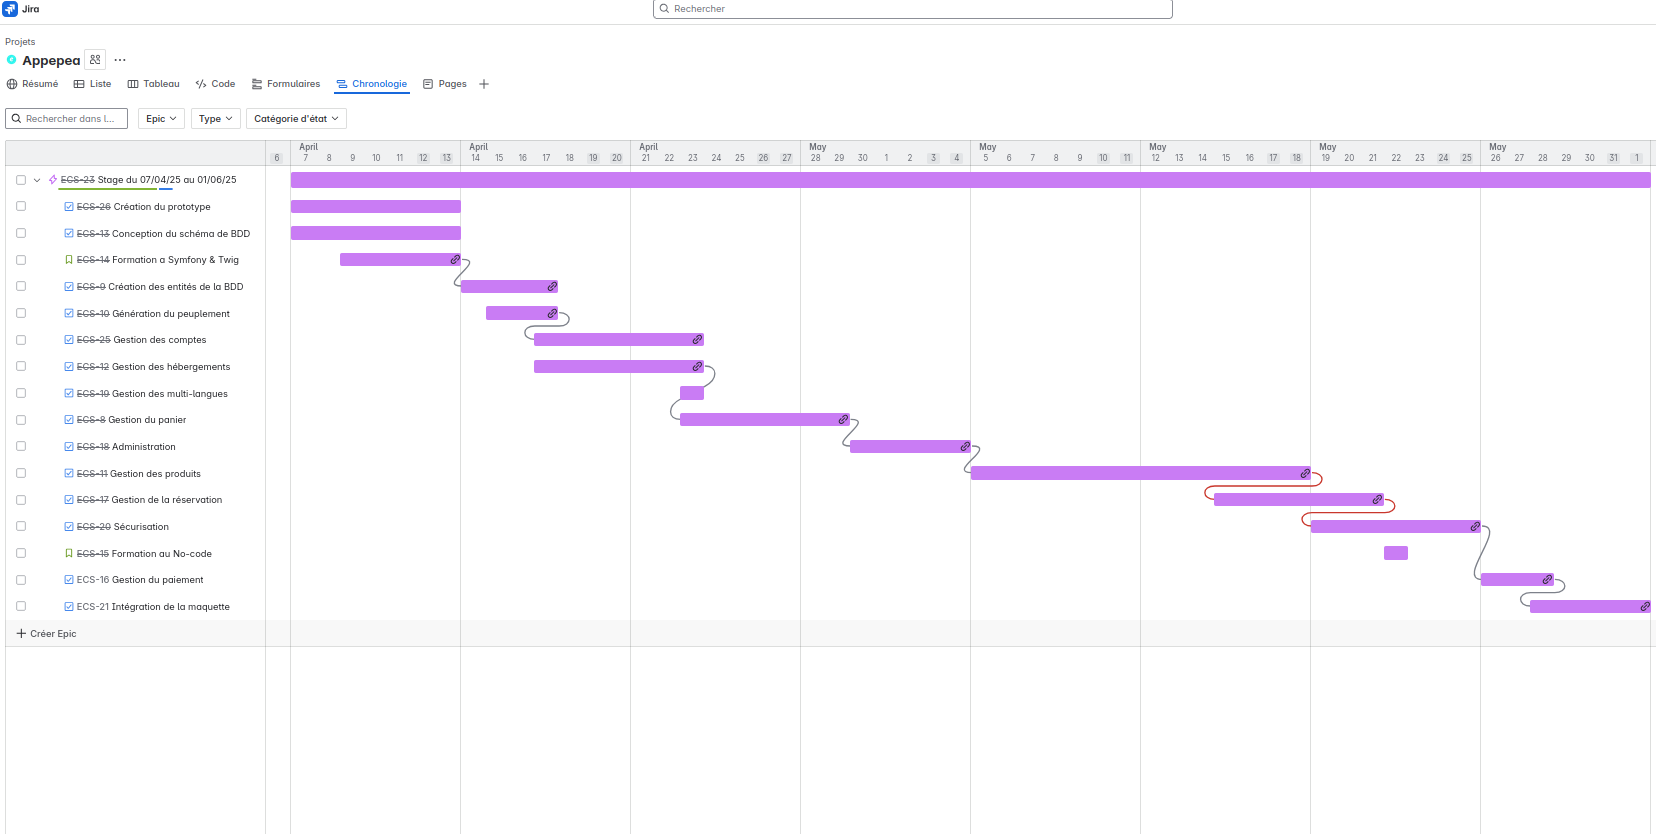
\includegraphics[height=5cm]{../img/gantt.png}
  				\caption{
    					\href{https://etudiant-team-z8ihahyp.atlassian.net/jira/software/projects/ECS/boards/1/timeline?timeline=WEEKS}{\underline{Diagramme Gantt}}.\\
    					\textit{Source : Mattéo Kervadec}
  				}
  				\label{fig:gantt}
			\end{figure}
		\end{minipage}
	\end{center}
	\vfill
\end{frame}

\planSlide{4}

% === REALISATIONS ===
\begin{frame}[label=realisation]{Solutions apportées aux projets}
	\begin{beamercolorbox}[wd=\paperwidth,ht=1.5em,dp=0.5em,leftskip=0.5cm]{section in head/foot}
  		\large \textbf{Réalisation 1 :} \normalsize Conception et modélisation de l'application
	\end{beamercolorbox}
	\vspace{0.5em}

	\begin{center}
  		\only<1> {
  			\begin{minipage}{0.9\textwidth}
  				\textbf{Situation :} Le projet manquait d’une structure claire pour organiser les données.\\
  				\textbf{Tâche :} Identifier les fonctionnalités de l'application.\\
  				\textbf{Action :}
  			  		\begin{itemize}
  						\item Identification des fonctionnalités
  						\item Réalisation du modèle conceptuel des données (MCD)
  						\item Création d'un prototype de l'application
  					\end{itemize}
				\textbf{Résultat :} Modèle clair et globale sur le fonctionnalité facilitant le développement backend.
			\end{minipage}
		}
		\only<2> {
			\begin{figure}[t]
  				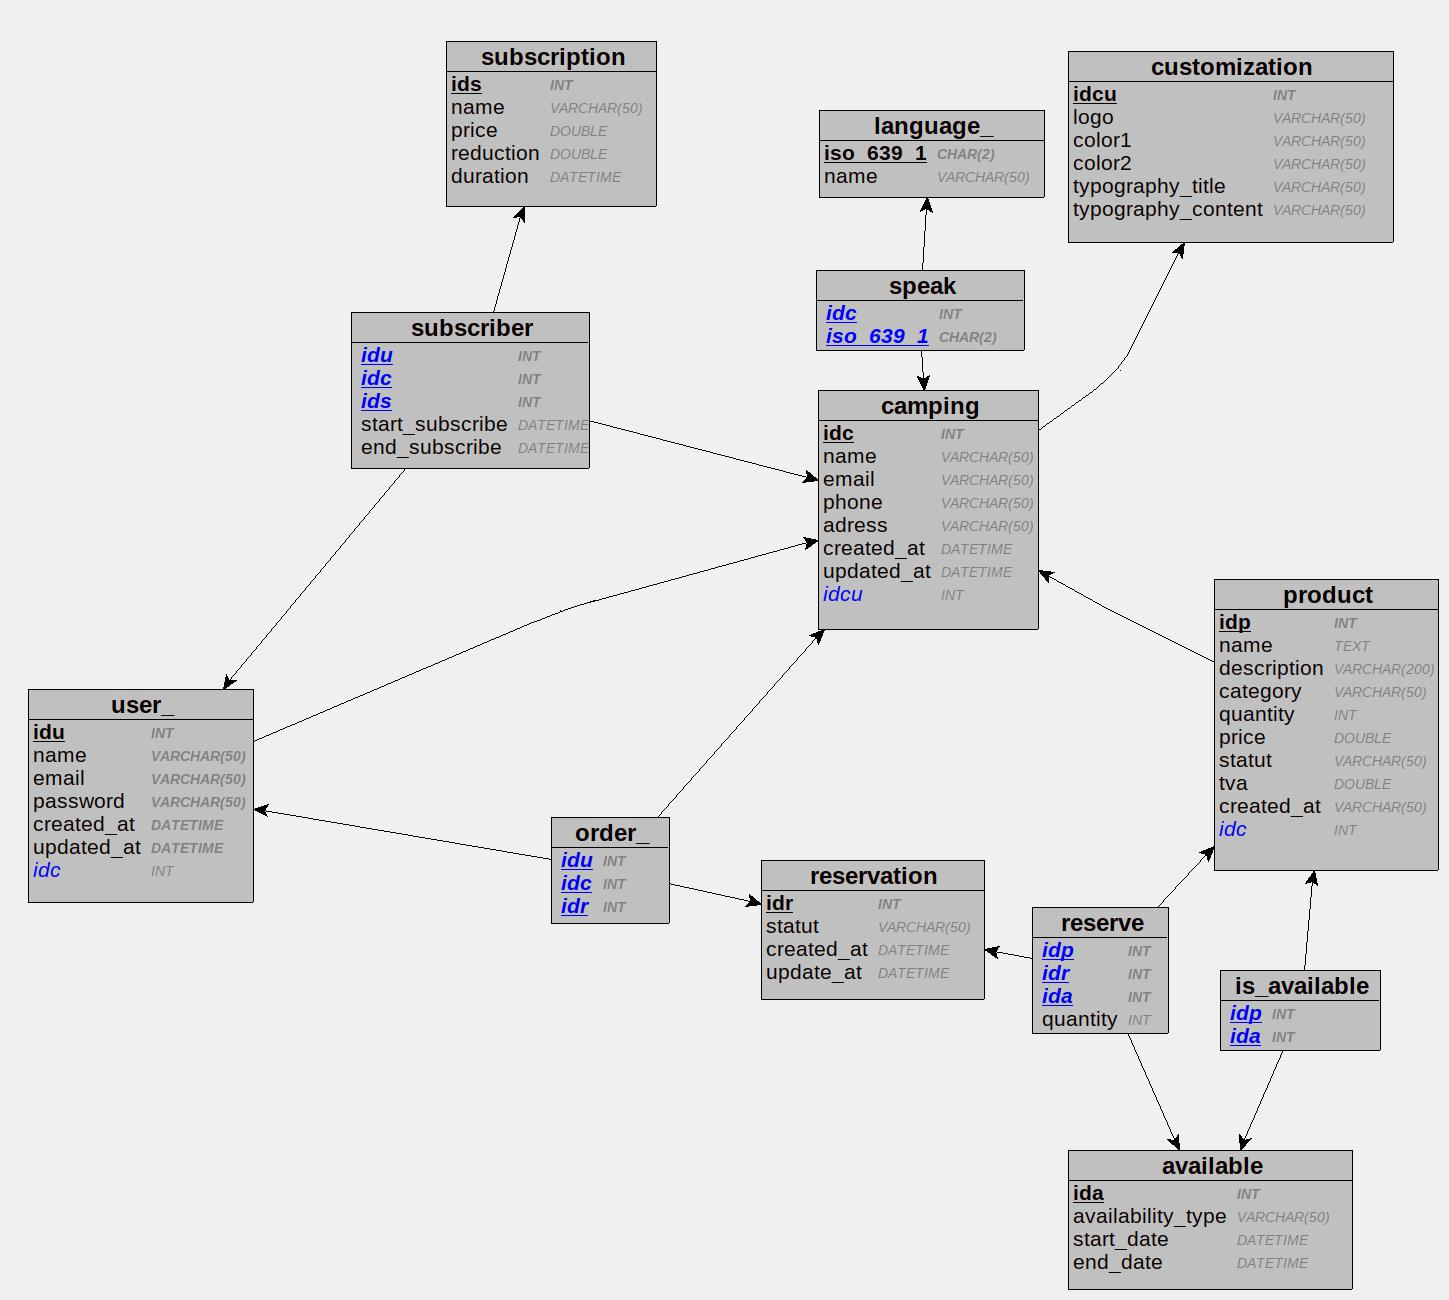
\includegraphics[height=5.5cm]{../img/conception/mcd_V1.jpg}
				\caption{	
					\centering			
  					\href{https://github.com/Matteo-K/Soutenance_E-delic/blob/main/img/conception/mcd_V1.jpg}{\underline{Modèle Conceptuel des données - version 1}}.\\
  					\textit{Source : Mattéo Kervadec}
				}
  				\label{fig:mcdV1}
  			\end{figure}
		}
		\only<3> {
			\addtocounter{figure}{1}
			\begin{figure}[t]
  				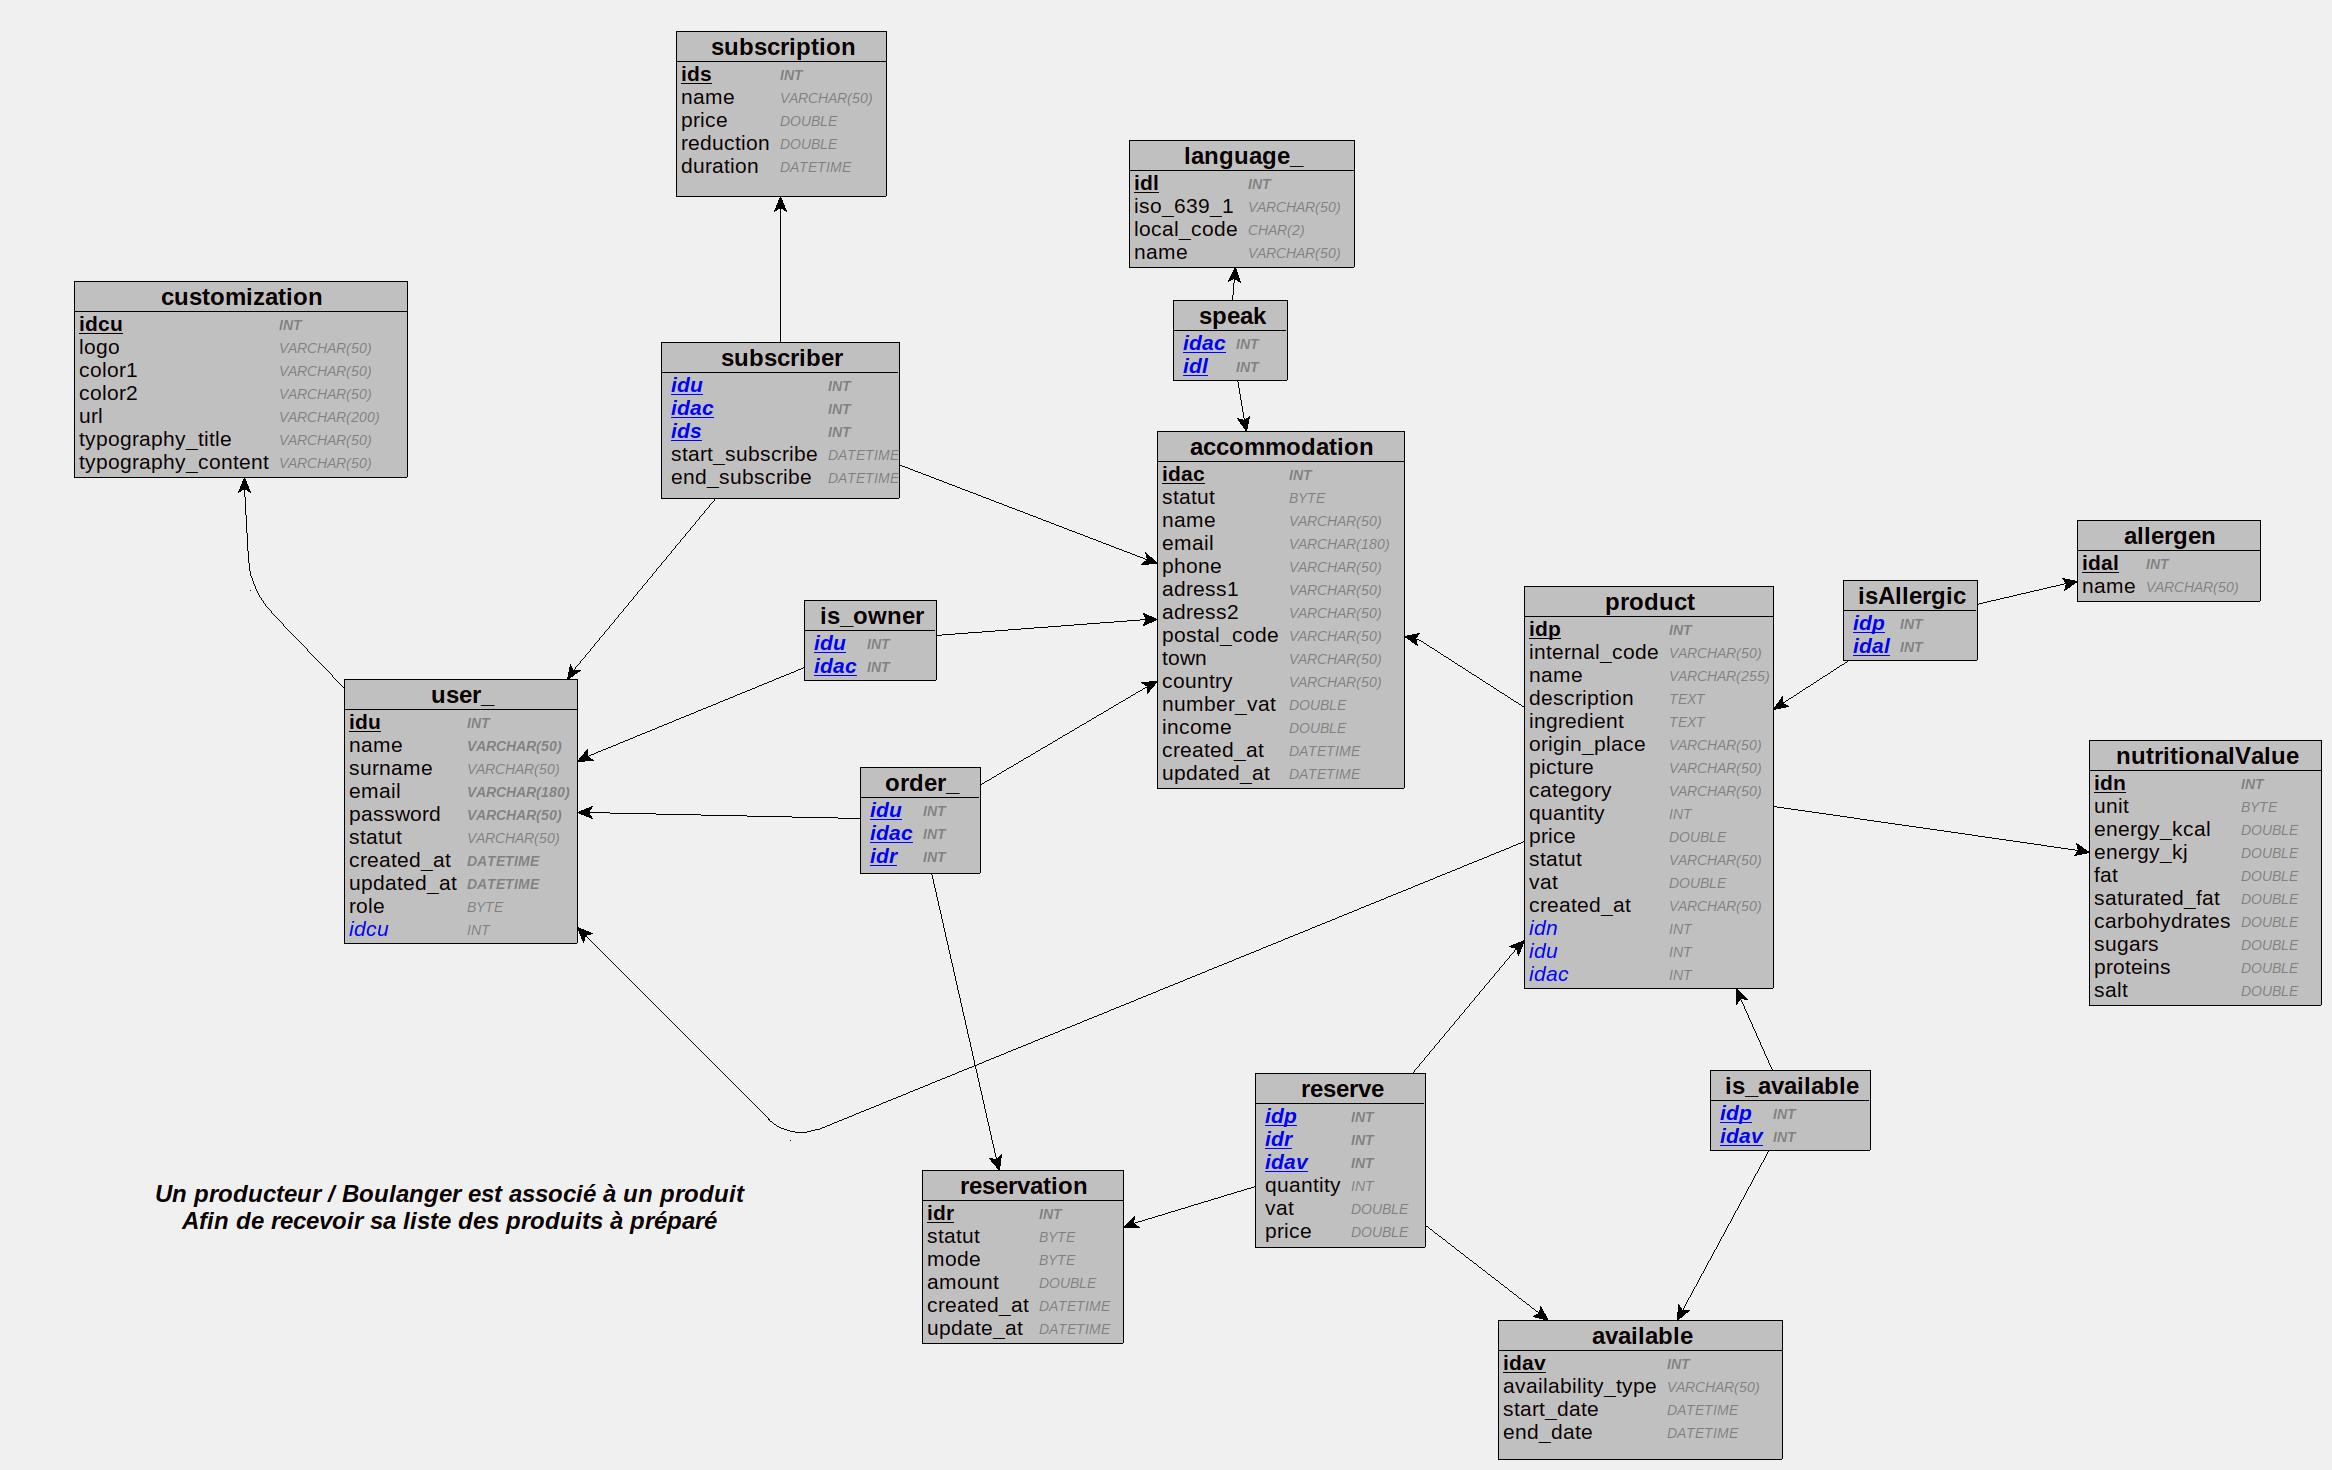
\includegraphics[height=5.5cm]{../img/conception/mcd_V2.jpg}
				\caption{	
					\centering			
  					\href{https://github.com/Matteo-K/Soutenance_E-delic/blob/main/img/conception/mcd_V2.jpg}{\underline{Modèle Conceptuel des données - version 2}}.\\
  					\textit{Source : Mattéo Kervadec}
				}
  				\label{fig:mcdV2}
  			\end{figure}
		}
		\only<4> {
			\addtocounter{figure}{2}
			\begin{figure}[t]
  				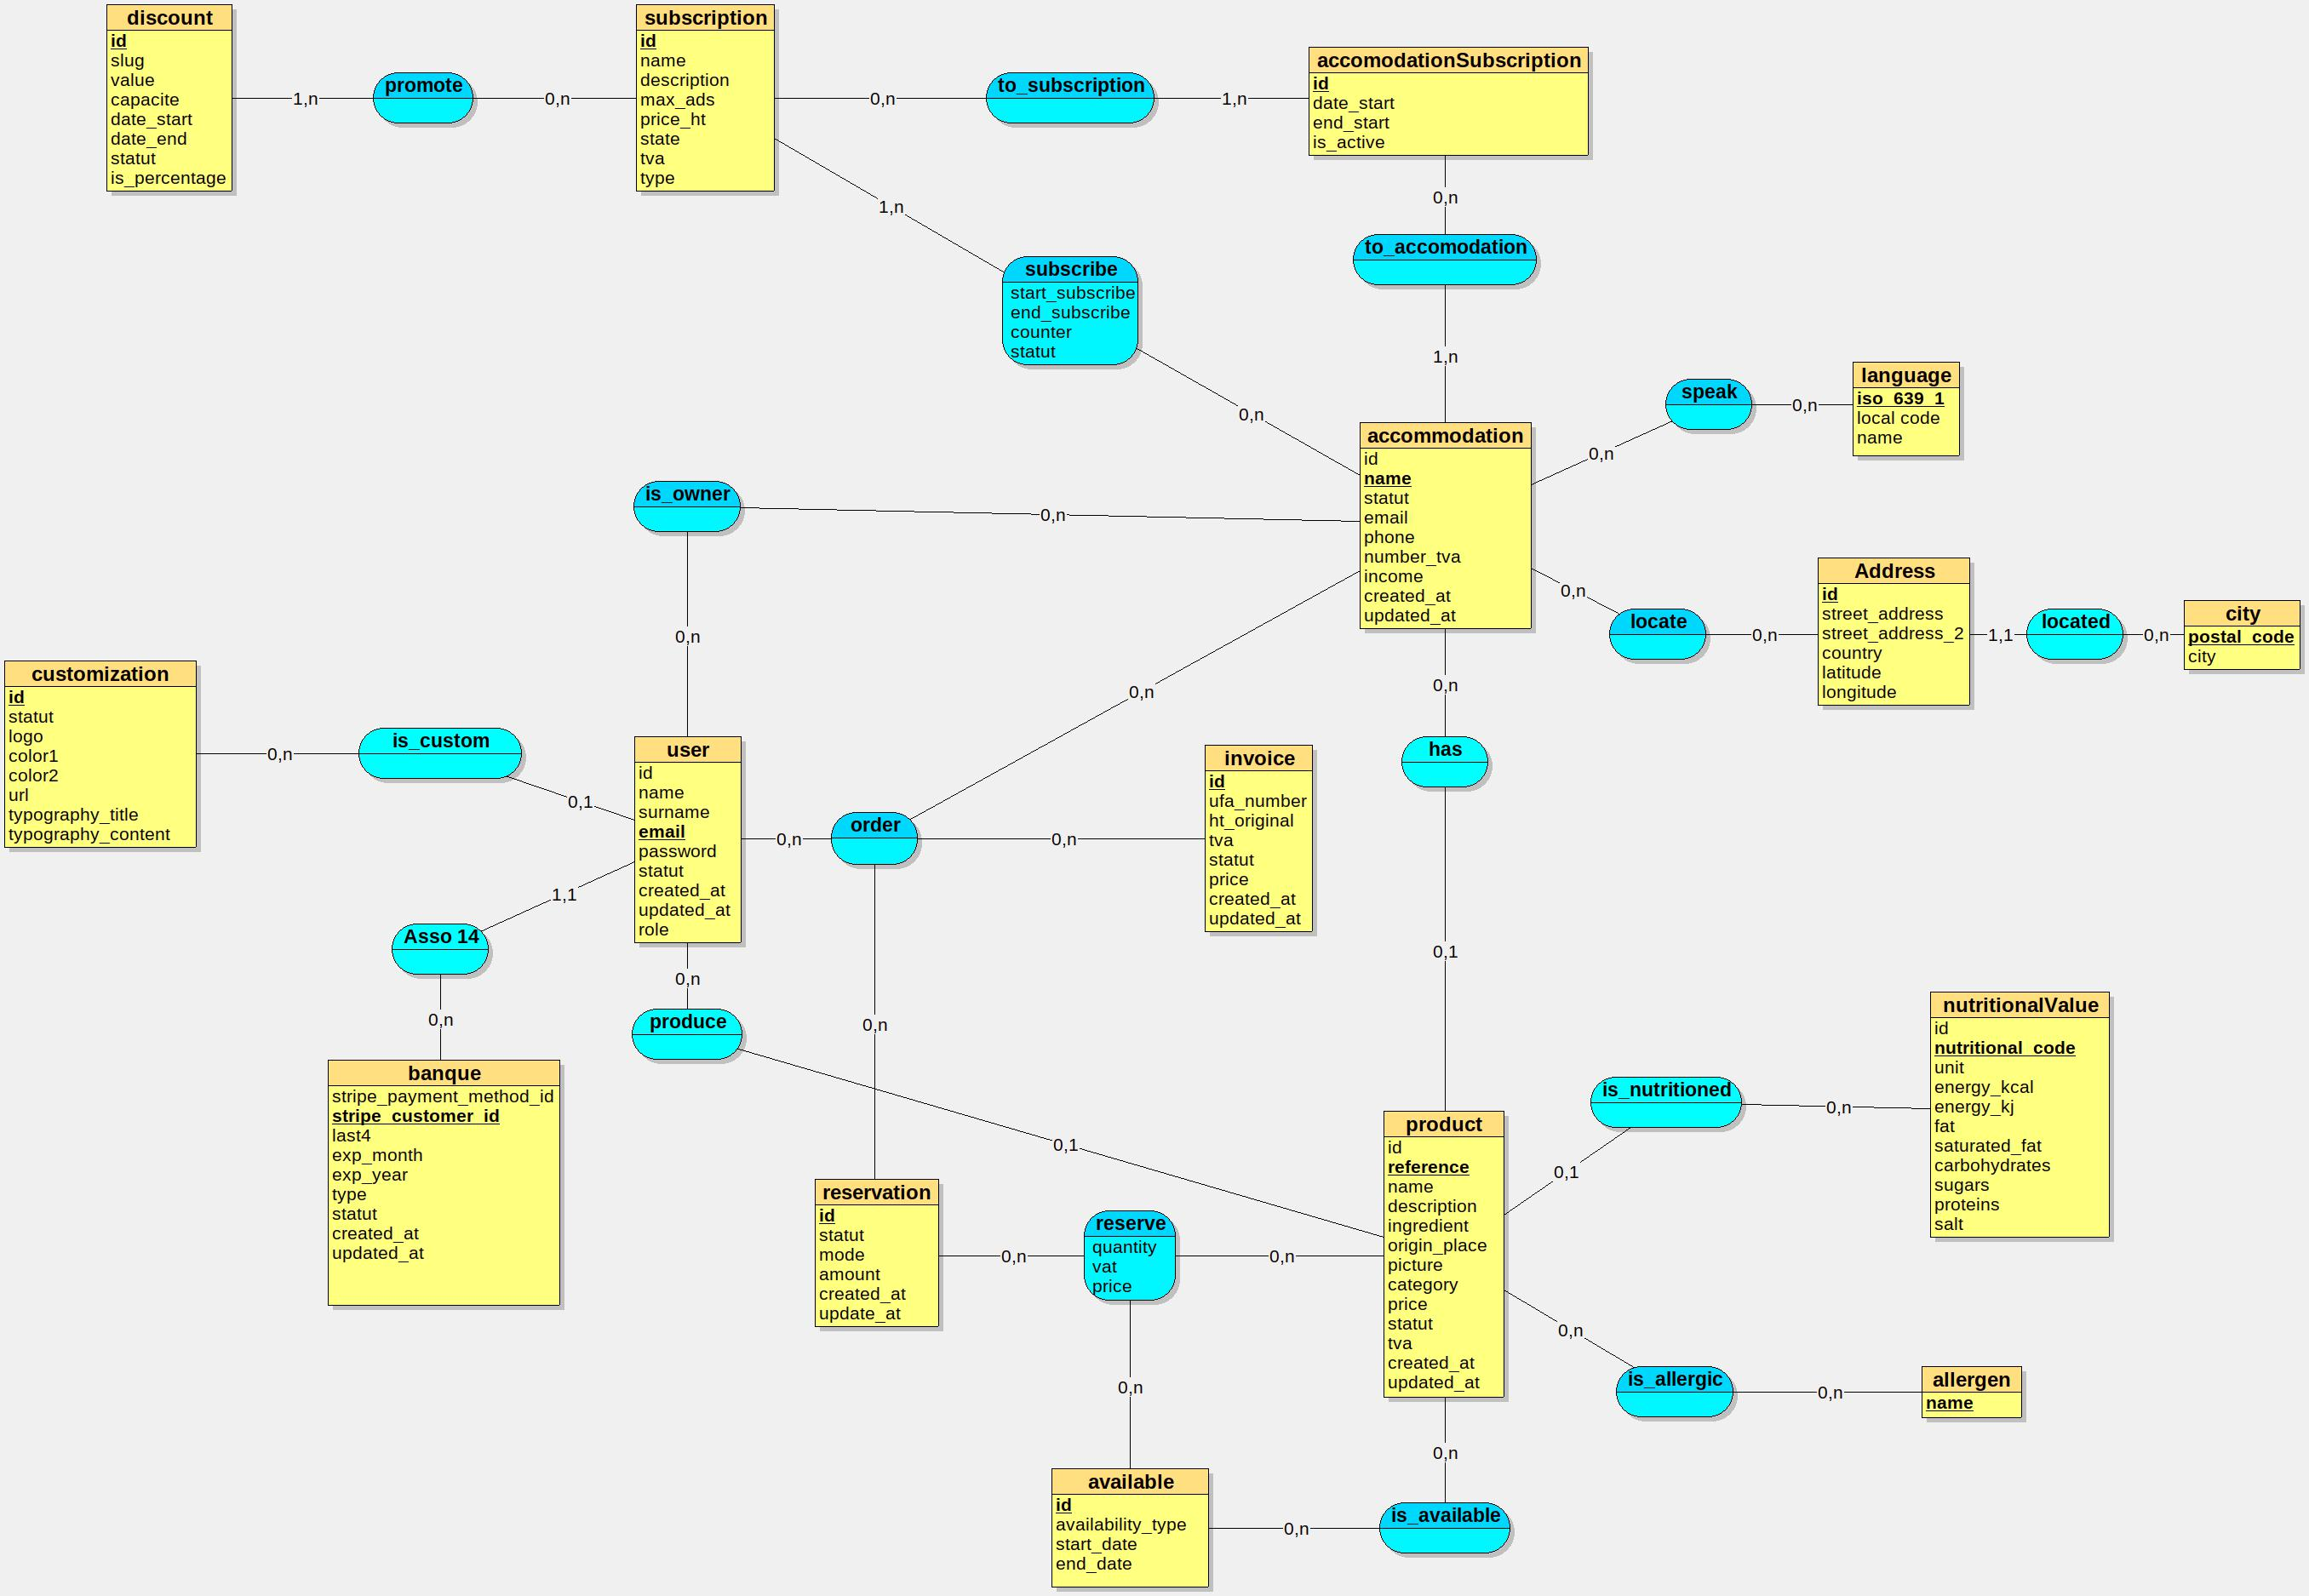
\includegraphics[height=5.5cm]{../img/conception/mcd_V3.jpg}
				\caption{	
					\centering			
  					\href{https://github.com/Matteo-K/Soutenance_E-delic/blob/main/img/conception/mcd_V3.jpg}{\underline{Modèle Conceptuel des données - version 3}}.\\
  					\textit{Source : Mattéo Kervadec}
				}
  				\label{fig:mcdV3}
  			\end{figure}
		}
		\only<5> {
			\addtocounter{figure}{3}
			\begin{figure}[t]
  				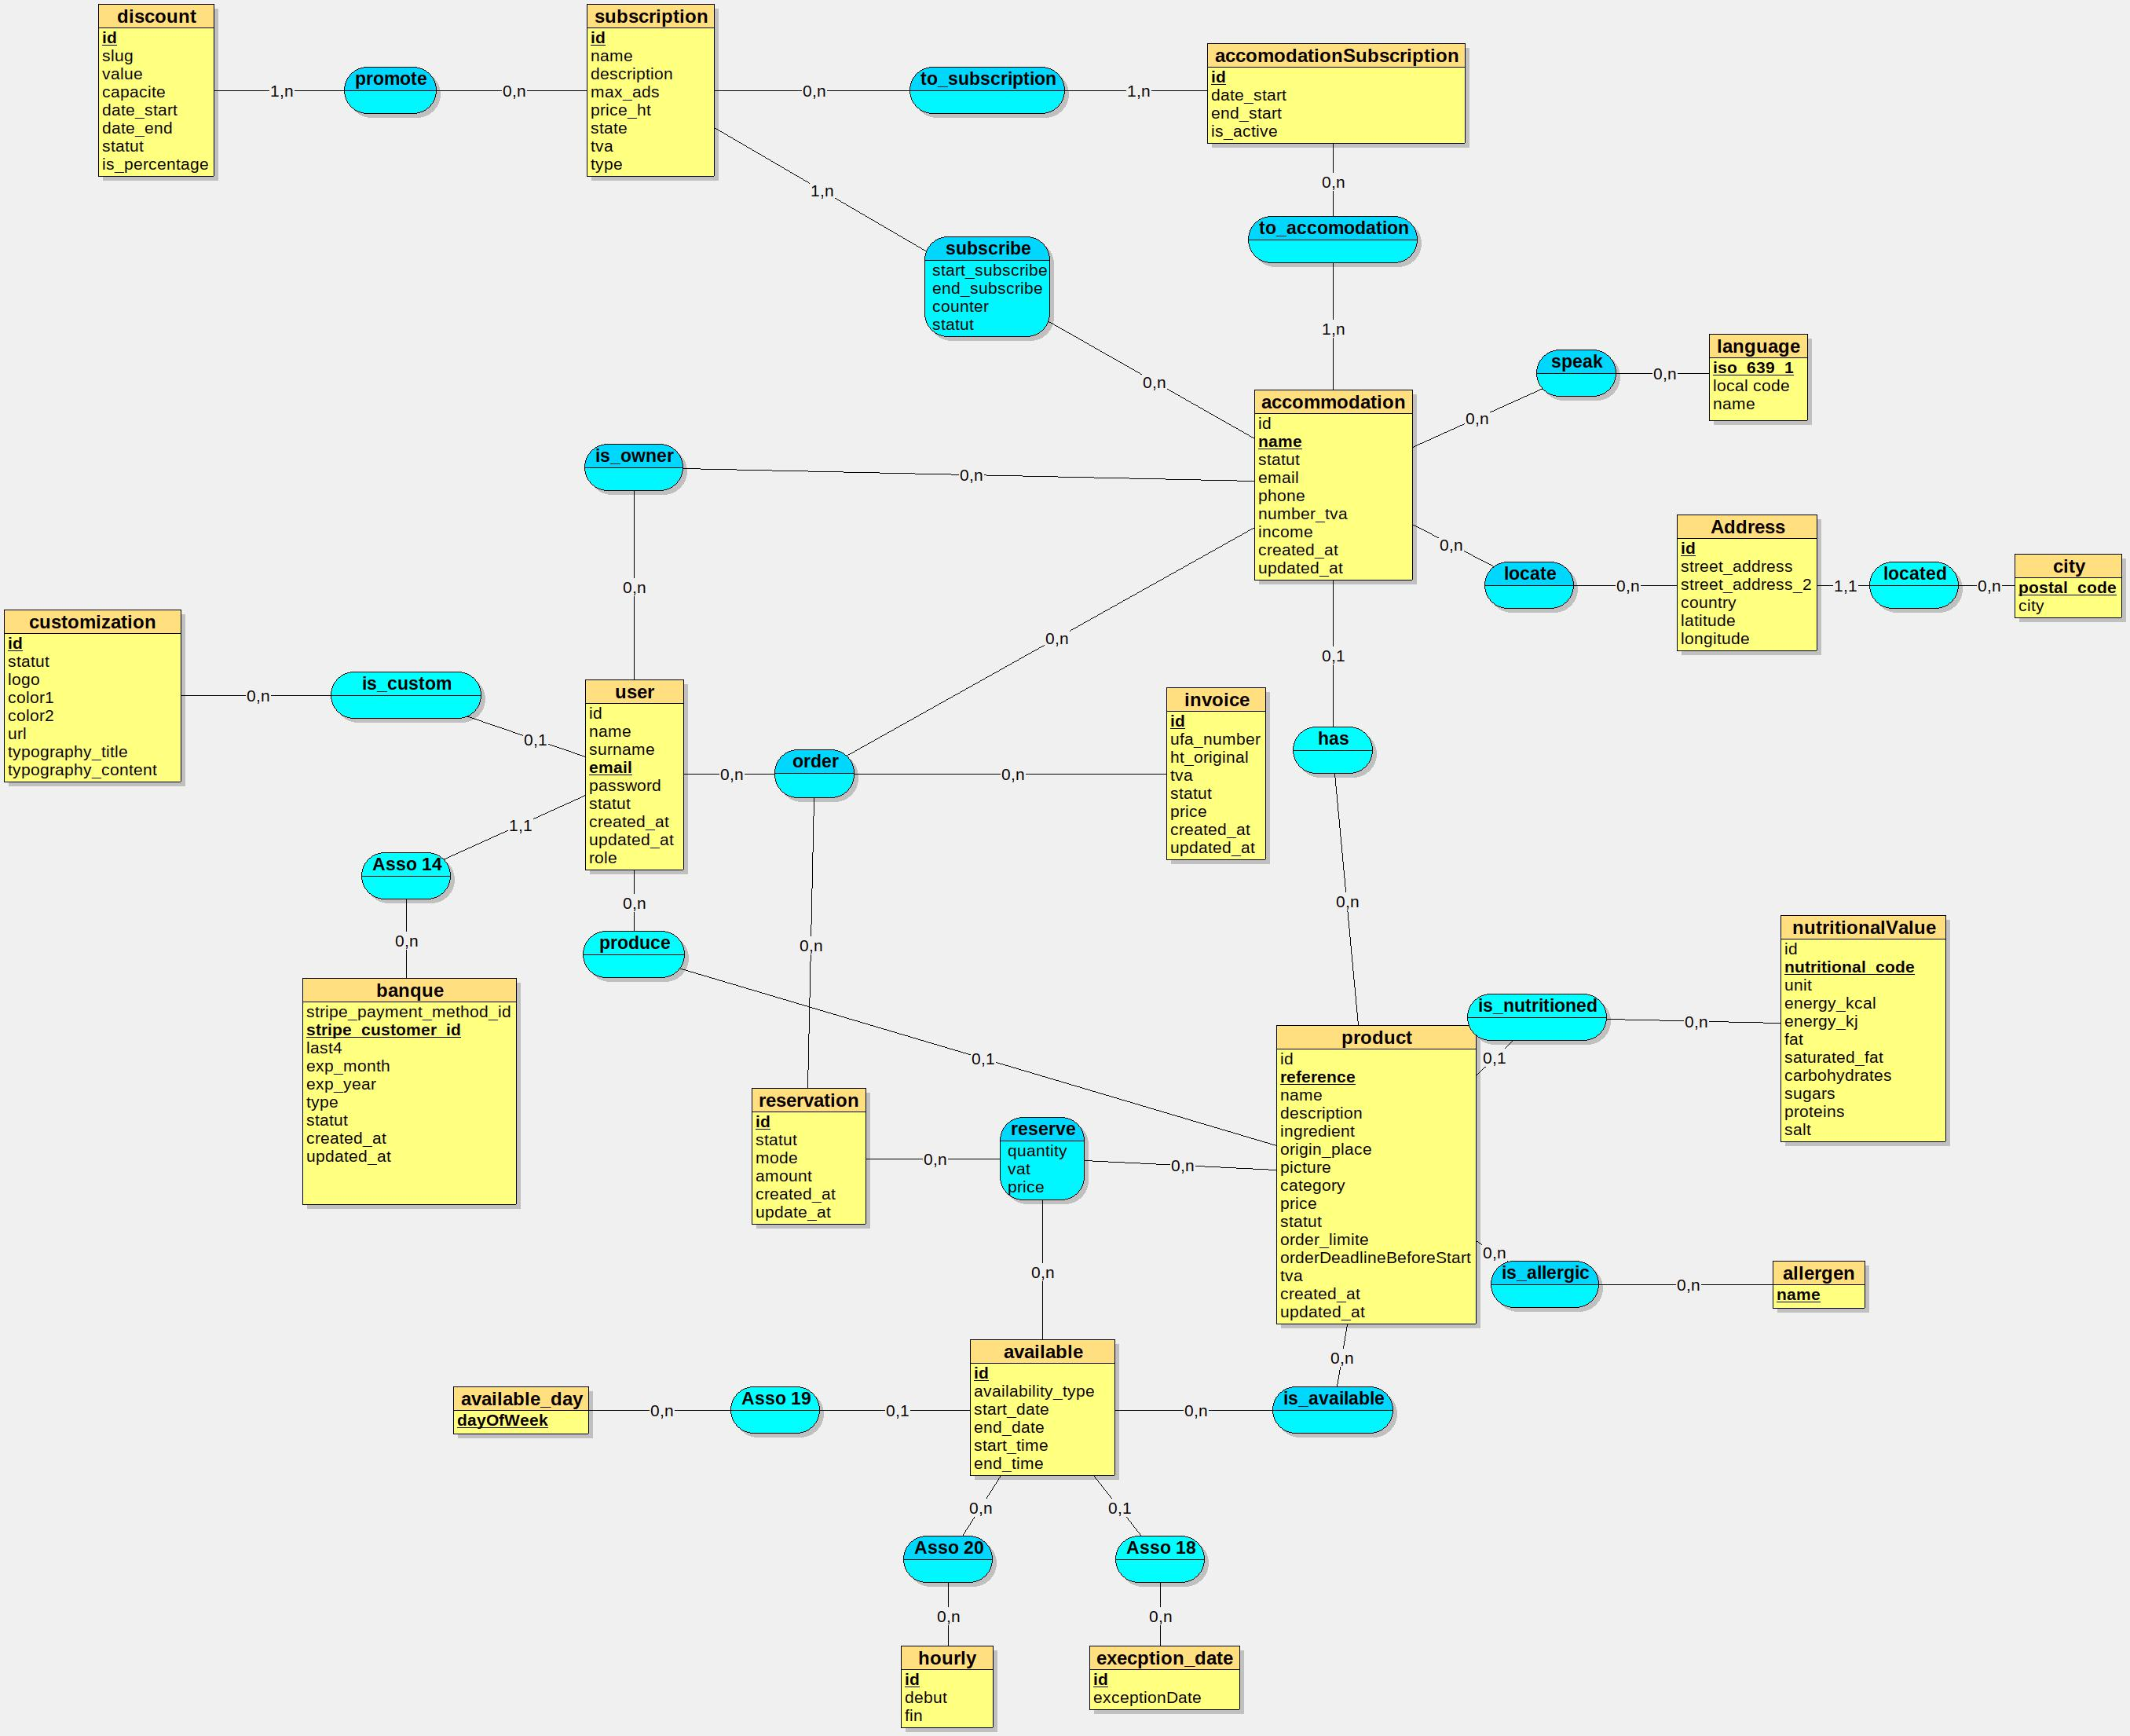
\includegraphics[height=5.5cm]{../img/conception/mcd_V4.jpg}
				\caption{	
					\centering			
  					\href{https://github.com/Matteo-K/Soutenance_E-delic/blob/main/img/conception/mcd_V4.jpg}{\underline{Modèle Conceptuel des données - version 4}}.\\
  					\textit{Source : Mattéo Kervadec}
				}
  				\label{fig:mcdV4}
  			\end{figure}
		}
		\only<6> {
			\addtocounter{figure}{4}
			\begin{figure}[t]
  				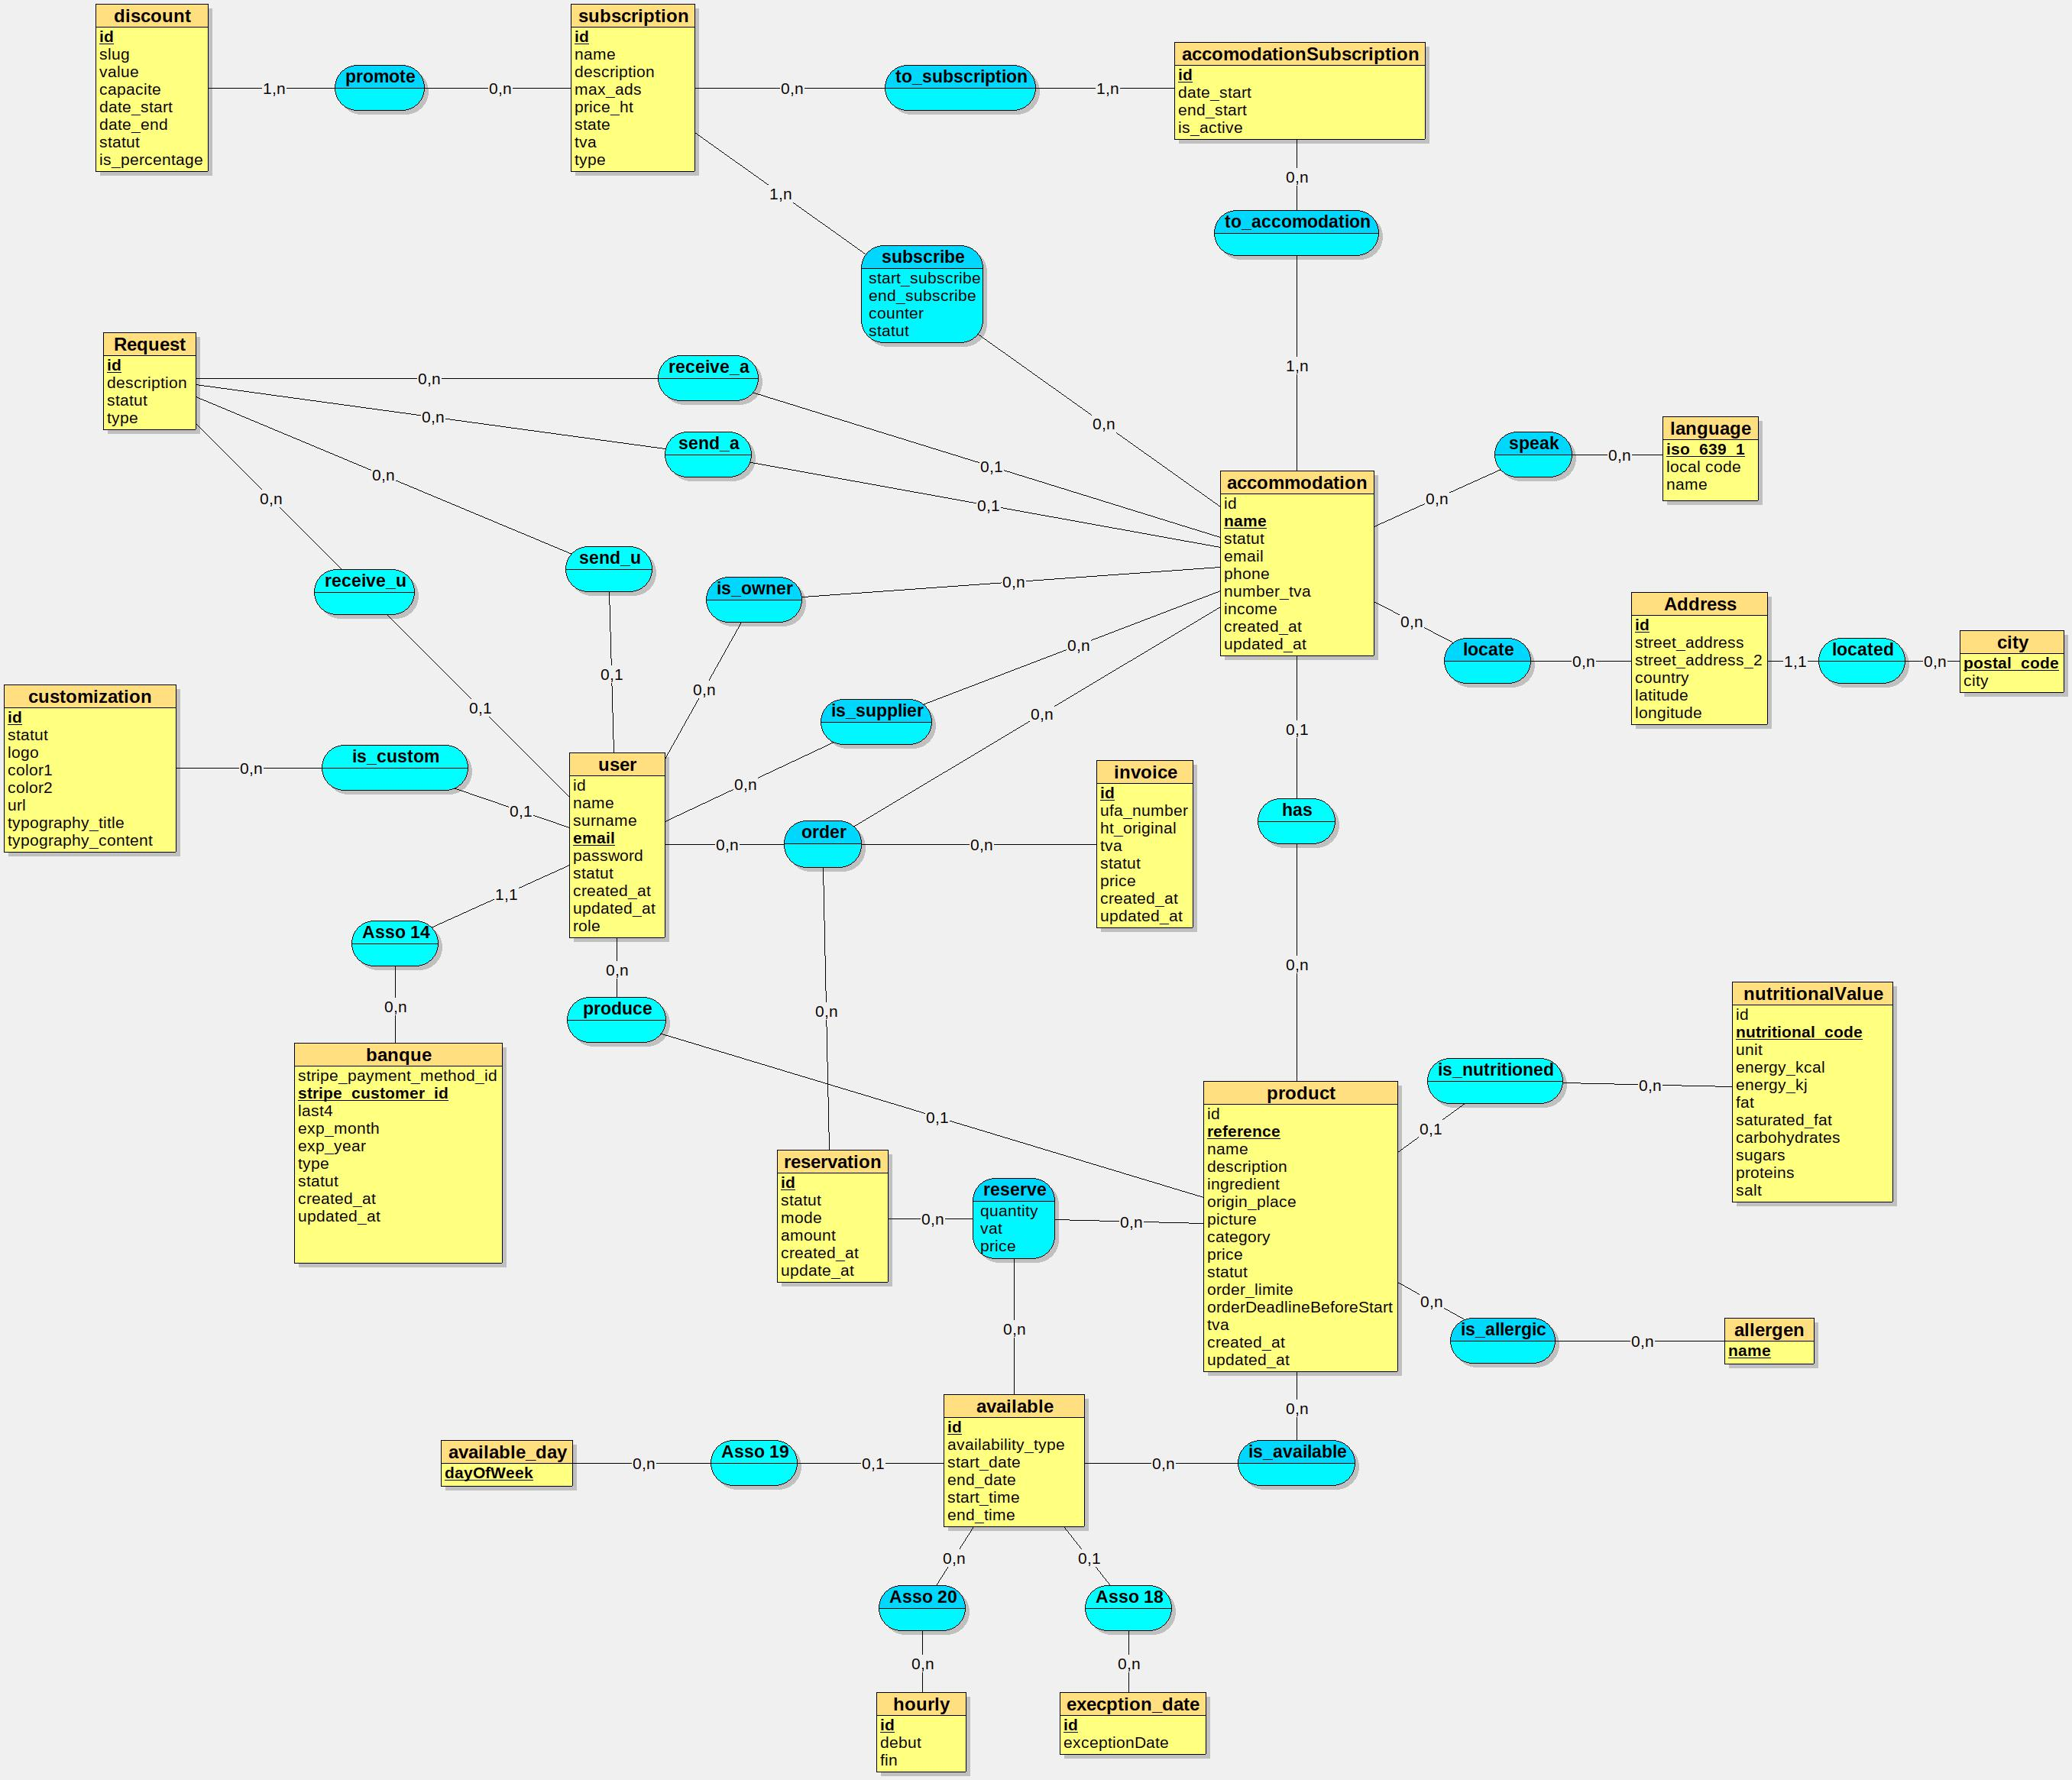
\includegraphics[height=5.5cm]{../img/conception/mcd_V5.jpg}
				\caption{	
					\centering			
  					\href{https://github.com/Matteo-K/Soutenance_E-delic/blob/main/img/conception/mcd_V5.jpg}{\underline{Modèle Conceptuel des données - version 5}}.\\
  					\textit{Source : Mattéo Kervadec}
				}
  				\label{fig:mcdV5}
  			\end{figure}
		}
	\end{center}
	\vfill
	\addtocounter{figure}{4}
\end{frame}

\begin{frame}{Solutions apportées aux projets}
	\begin{beamercolorbox}[wd=\paperwidth,ht=1.5em,dp=0.5em,leftskip=0.5cm]{section in head/foot}
  		\large \textbf{Réalisation 2 :} \normalsize Gestion des comptes et des rôles utilisateur
	\end{beamercolorbox}
	\vspace{0.5em}
	\begin{center}
  		\begin{minipage}{0.9\textwidth}
  			\textbf{Situation :} Tout les utilisateurs ont un accès libre au service.\\
  			\textbf{Tâche :} Gestion des rôles et authentification.\\
  			\textbf{Action :} Mises en places de sécurités.
  				\begin{itemize}
  					\item Authentification avec JWT Tokens
  					\item Controlle d'accès (Security \& Voter)
  					\item Usurpation des utilisateurs (Admin)
  				\end{itemize}
			\textbf{Résultat :}
				\begin{itemize}
					\item Multi-accès sécurisé à la plateforme
					\item Fonctionnalités adaptées selon les rôles de l'utilisateur
				\end{itemize}
  		\end{minipage}
	\end{center}
	\vfill
\end{frame}

\begin{frame}{Solutions apportées aux projets}
	\begin{beamercolorbox}[wd=\paperwidth,ht=1.5em,dp=0.5em,leftskip=0.5cm]{section in head/foot}
  		\large \textbf{Réalisation 3 :} \normalsize Développement de la logique métier e-commerce
	\end{beamercolorbox}
	\vspace{0.5em}
	\begin{center}
  		\begin{minipage}{0.9\textwidth}
  			\textbf{Situation :} Plateforme sans fonctionnalité de commande ou panier.\\
  			\textbf{Tâche :} Sélectionner un produit suivant sa disponibilité.\\
  			\textbf{Action :}
				\begin{itemize}
					\item Gestion des produits
					\item Gestion du panier (API REST)
					\item Implémentation d'un service de disponibilité
				\end{itemize}
			\textbf{Résultat :} Création et sélection de produit fluide et dynamique.
  		\end{minipage}
	\end{center}
	\vfill
\end{frame}

\begin{frame}{Solutions apportées aux projets}
	\begin{beamercolorbox}[wd=\paperwidth,ht=1.5em,dp=0.5em,leftskip=0.5cm]{section in head/foot}
  		\large \textbf{Réalisation 4 :} \normalsize Mise en place de la procédure de paiement et réservation
	\end{beamercolorbox}
	\vspace{0.5em}
	\begin{center}
  		\begin{minipage}{0.9\textwidth}
  			\textbf{Situation :} Conclure la procédure de gestion.\\
  			\textbf{Tâche :} Volonté d'encaisser et retracer les commandes.\\
  			\textbf{Action :}
  				\begin{itemize}
  					\item Integration de stripe pour les paiements sécurisés
  					\item Mise en place d'historique de commande
  				\end{itemize}
			\textbf{Résultat :} Traçage et méthode de paiement fonctionnel qui nécessiterait des améliorations.
				\begin{itemize}
					\item Porte-monnaie virtuelle
					\item Gestion de suivi de livraison
				\end{itemize}
  		\end{minipage}
	\end{center}
	\vfill
\end{frame}

\planSlide{5}

% === CONCLUSION ===
\begin{frame}[label=conclusion]{Conclusion}
  	\begin{beamercolorbox}[wd=\paperwidth,ht=1.5em,dp=0.5em,leftskip=0.5cm]{section in head/foot}
  		\large \textbf{Bilan de la situation}
	\end{beamercolorbox}
	\vspace{0.5em}
	\begin{center}
  		\begin{minipage}{0.9\textwidth}
	  		Objectifs atteints, quelques améliorations possibles.
  			\begin{itemize}
  				\item Base de Site e-commerce fonctionnel
			  	\item Manque plus que le design
			  	\item Ajouté des fonctionnalité : 
			  	\begin{itemize}
			  		\item Porte-monnaie
			  		\item Gestion d'abonnement
			  	\end{itemize}
			\end{itemize}
  		\end{minipage}
	\end{center}
	\vfill
\end{frame}

\begin{frame}{Conclusion}
  	\begin{beamercolorbox}[wd=\paperwidth,ht=1.5em,dp=0.5em,leftskip=0.5cm]{section in head/foot}
  		\large \textbf{Bilan technique}
	\end{beamercolorbox}
	\vspace{0.5em}
	\begin{center}
  		\begin{minipage}{0.9\textwidth}
  			\begin{itemize}
  				\item Base de Site e-commerce fonctionnel
			  	\item Manque plus que le design
			  	\item Ajouté des fonctionnalité : 
			  	\begin{itemize}
			  		\item Porte-monnaie
			  		\item Gestion d'abonnement
			  	\end{itemize}
			\end{itemize}
  		\end{minipage}
	\end{center}
	\vfill
\end{frame}

\begin{frame}{Conclusion}
  	\begin{beamercolorbox}[wd=\paperwidth,ht=1.5em,dp=0.5em,leftskip=0.5cm]{section in head/foot}
  		\large \textbf{Bilan humain}
	\end{beamercolorbox}
	\vspace{0.5em}
	\begin{center}
  		\begin{minipage}{0.9\textwidth}
  			\begin{itemize}
  				\item
  			\end{itemize}
  		\end{minipage}
	\end{center}
	\vfill
\end{frame}

\begin{frame}[label=remerciements]{\Large Remerciements}
    \logoEdeclic
    \begin{center}
        \vspace{1em}
        \begin{minipage}{0.9\textwidth}
        		Un grand merci à toute l'équipe de \textbf{e-declic} et mon tuteur de stage \textbf{Michel Morvant} pour l'accueil et leurs accompagnements durant ce stage. \vspace{0.25cm} \\
            Merci à l'\textbf{IUT de Lannion} pour m'avoir offert cette opportunité de formation. \vspace{0.25cm} \\
            Je remercie également \textbf{le jury} pour le temps accordé et l'intérêt porté à mon travail. \vspace{0.25cm} \\
            Enfin, je suis heureux de pouvoir poursuivre cette expérience chez \textbf{e-declic} en \textbf{alternance dès cet été}.
        \end{minipage}
    \end{center}
    \vfill
\end{frame}

\begin{frame}[label=sources]{Sources}
	\begin{itemize}
		\item \href{https://www.e-declic.com/}{lien} - Site web E-declic
		\item \href{https://www.francenum.gouv.fr/activateurs/e-declic}{lien}
		\item \href{https://annuaire-entreprises.data.gouv.fr/entreprise/e-declic-453413296}{lien}
		\item \href{https://entreprises.lefigaro.fr/e-declic-56/entreprise-453413296}{lien}
	\end{itemize}

\end{frame}

\end{document}